\section{Алгоритм определения стабилизации состояния системы} % (fold)
\label{sec:StabilityAlgorithm}
    Важным вопросом, на который необходимо обратить внимание, это вопрос о том, является ли полученное состояние системы достаточно стабильным. Обычно, предполагается что время релаксации должно значительно превышать число частиц, и потому прежде чем снимать результаты, предварительно проводится длительная симуляция системы на протяжении $10^5 \div 6$ шагов по времени.

    Как уже было сказано, мы предполагаем такой подход расточительным, и потому нами предложено использовать простой критерий релаксации системы. Как известно из термодинамики, влияние флуктуаций на параметры системы пропорционально $1/\sqrt{N}$, где $N$ - число частиц. Потому мы предложили выполнять для начала 100 шагов по времени для каждого значения шума, а затем, если разница средней скорости и средней скорости на предыдущей итерации \textit{НЕ} оказывается меньше чем $1/\sqrt{N}$, продолжать симуляцию с тем же значением шума (см. алгоритм на рис.~\ref{fig:MainAlgorithm})

    \begin{figure}[h]
    \centering
        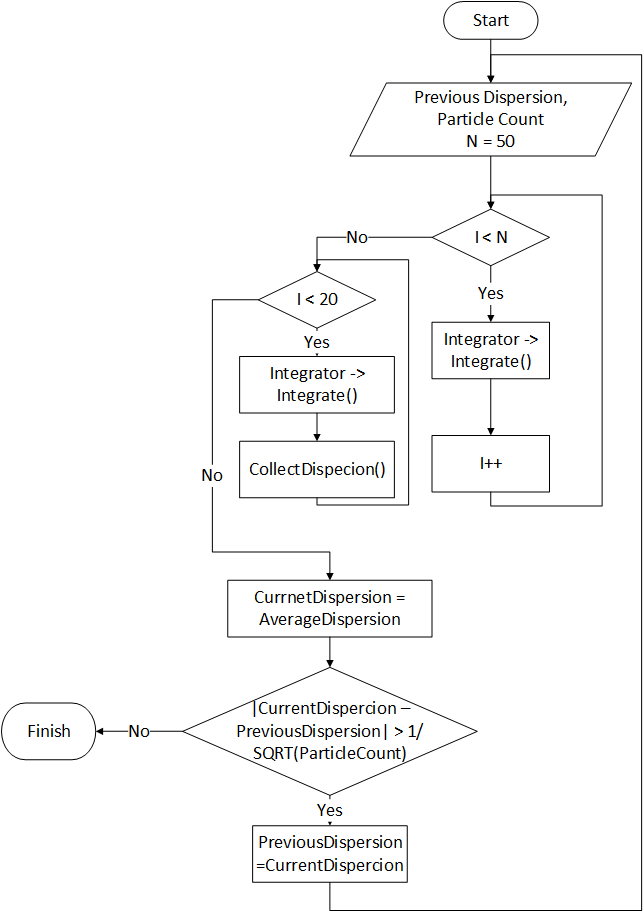
\includegraphics[width = \textwidth]{Images/MainAlgorithm}
        \caption{Алгоритм определения стабильного состояния системы}
        \label{fig:MainAlgorithm}
    \end{figure}

% subsection ViksecModelProgramm (end)